
%
\section{Application:  Stochastic Submodular Coverage}
\label{sec:stochastic-set-cover} 
%

Suppose that instead of wishing to adaptively place $\budget$ unreliable sensors
to maximize
the utility of the information obtained, as discussed
in~\secref{sec:stochastic-maximization}, 
we have a quota on utility and wish to adaptively place the minimum number of
unreliable sensors to achieve this quota. This amounts to  
a minimum-cost coverage version of the
Stochastic Submodular Maximization problem introduced
in~\secref{sec:stochastic-maximization}, which we call 
\emph{Stochastic Submodular Coverage}.

As in~\secref{sec:stochastic-maximization}, in the Stochastic Submodular Coverage  problem we suppose there is a function 
$\hat{f}:2^{\groundset\times\outcomes}\to \NonNegativeReals$ which quantifies
the utility of a set of sensors in arbitrary states.
Also, the states of each sensor are independent, so that 
$\Pr{\rvrlz = \rlz} = \prod_{\elem \in \groundset} \Pr{\rvrlz(\elem) =  \rlz(\elem)}$.
The goal is to obtain a quota $Q$ of utility at minimum cost.
Thus, we define our objective as
$f(A,\rlz) := \min\set{Q,\hat{f}(\set{(\elem,\rlz(\elem)) : \elem \in A})}$, and want to 
find a policy $\policy$ covering every realization 
and minimizing
$\cavg{\policy} := \expct{|\played{\policy}{\rvrlz}|}$.
We additionally assume that this quota can always be obtained using
sufficiently many sensor placements; formally, this amounts to $f(E, \rlz) = Q$ for all $\rlz$.
We obtain the following result, whose proof we defer until the end of this section.

\begin{theorem} \label{thm:stochastic-submodular-cover}
Fix a prior with independent sensor states so that $\Pr{\rvrlz = \rlz} = \prod_{\elem \in \groundset} \Pr{\rvrlz(\elem) =  \rlz(\elem)}$,
and let %
$\hat{f}:2^{\groundset\times\outcomes} \to \NonNegativeReals$
be a monotone submodular function.
Fix $Q \in \NonNegativeReals$ such that 
$f(A, \rlz) := \min \paren{Q,\ \hat{f}(\set{(\elem,\rlz(\elem)) : \elem \in A})}$
satisfies  $f(E, \rlz) = Q$ for all $\rlz$.
Let $\eta$ be any value such that 
$f(S, \rlz) > Q - \eta$ implies $f(S, \rlz) = Q$ for all $S$ and $\rlz$.
Finally, let $\policy$ be an $\alpha$-approximate greedy policy for maximizing
$f$, and let $\policy^*$ be any policy.  Then 
\[
\acst{\policy} \le  \alpha\,
\acst{\policy^*}\paren{\ln \paren{\frac{Q}{\eta}} + 1} \mbox{.}
\]
\end{theorem}

\subsection{A Special Case: The Stochastic Set Coverage Problem}
The Stochastic Submodular Coverage problem is a generalization of the 
\emph{Stochastic Set Coverage} problem~\citep{goemans06stochastic}. 
In Stochastic Set Coverage the underlying
submodular objective $\hat{f}$ is the number of elements covered in
some input set system.  In other words, there is a ground set $U$ of
$n$ elements to be covered, and items $\groundset$ such that each item
$\elem$ is associated with a distribution over subsets of $U$.  When
an item is selected, a set is sampled from its distribution, as
illustrated in \figref{fig:stocsetcover}.  The
problem is to adaptively select items until all elements of $U$
are covered by sampled sets, 
while minimizing the expected number of items selected.
Like us, 
\citeauthor{goemans06stochastic} also assume that 
the subsets are sampled independently for each item,  
and every element of $U$ can
be covered in every realization, so that $f(\groundset, \rlz) =
|U|$ for all $\rlz$.

 \begin{figure}%
 \centering 
 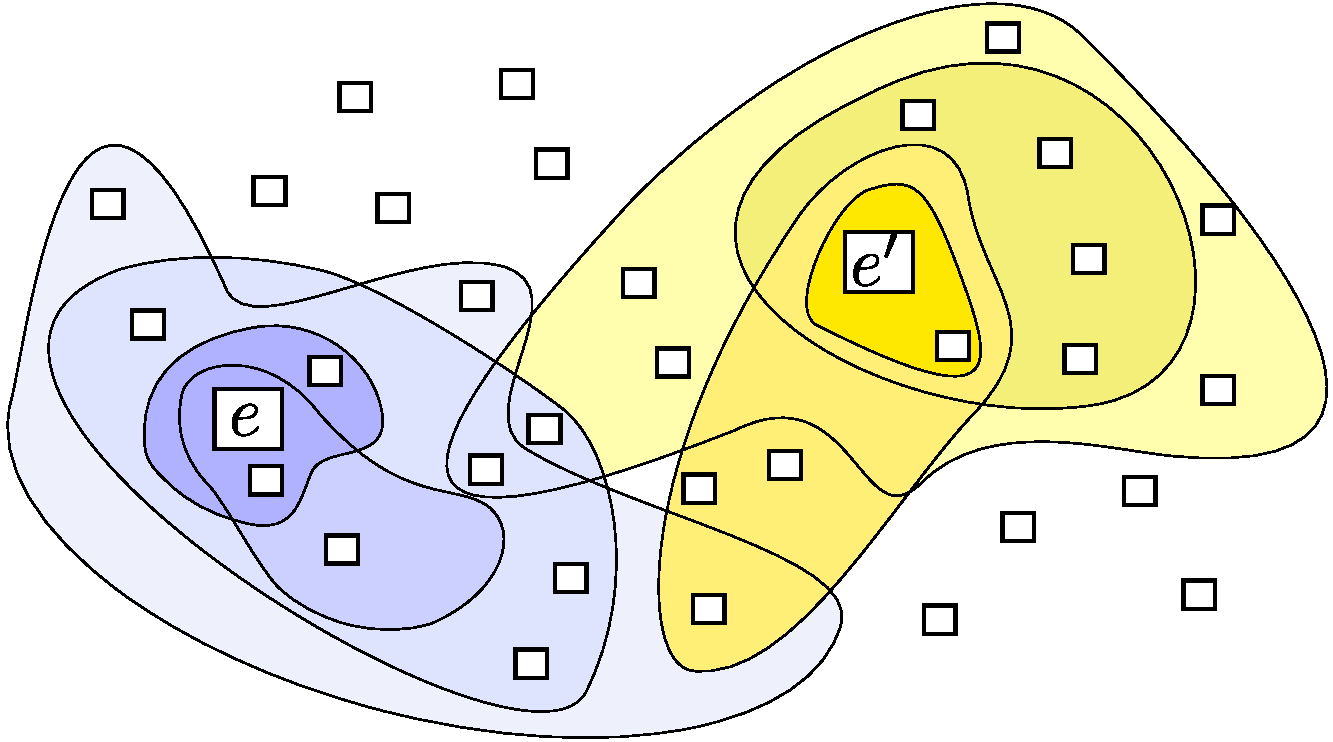
\includegraphics[height=4.5cm]{figs/stocSetCover}
 \caption{Illustration of part of a Stochastic Set Cover instance.  Shown are
   the supports of two distributions over sets, indexed by items $e$ (marked in blue) and $e'$ (yellow).   \label{fig:stocsetcover}}
 \end{figure} 

\citeauthor{goemans06stochastic} primarily
investigated the adaptivity gap (quantifying how much adaptive policies can outperform non-adaptive policies) of Stochastic Set Coverage, for variants in which
items can be repeatedly selected or not, and prove adaptivity gaps of
$\Theta(\log n)$ in the former case, and between $\Omega(n)$ and
$\cO(n^2)$ in the latter.  They also provide an $n$-approximation
algorithm.
%
More recently, \citet{liu08near} considered a special case of
Stochastic Set Coverage in which each item may be in one of two
states.  
They were motivated by a streaming database problem, in which a
collection of queries sharing common filters must all be evaluated on
a stream element.  They transform the problem to a Stochastic Set
Coverage instance in which (filter, query) pairs are to be covered by filter
evaluations;  which pairs are covered by a filter depends on the
(binary) outcome of evaluating it on the stream element.  
The resulting instances satisfy the assumption that 
every element of $U$ can be covered in every realization. 
They study, among other algorithms, the adaptive greedy algorithm
specialized to this setting, and show that if 
the subsets are sampled independently for each item, so that 
$\prob{\rvrlz = \rlz} = \prod_{\elem} \prob{\rvrlz(\elem) = \rlz(\elem)}$,
then it is an $\mathcal{H}_{n} := \sum_{x=1}^{n} \frac{1}{x}$
approximation.
(Recall $\ln(n) \le \mathcal{H}_{n} \le \ln(n)+1$ for all $n \ge 1$.)  
Moreover,  \citeauthor{liu08near} report that it
empirically outperforms a number of other algorithms in their experiments.

The \term submodularity framework allows us to recover \citeauthor{liu08near}'s 
result, and 
generalize it to richer item distributions over subsets of $U$, all as a corollary of \thmref{thm:stochastic-submodular-cover}.
Specifically, we obtain a $(\ln(n) + 1)$-approximation for the Stochastic Set Coverage problem, where $n := |U|$, which matches the approximation ratio for the greedy algorithm for classical Set Cover that 
Stochastic Set Coverage generalizes.
Like \citeauthor{liu08near}'s result,
our result is tight if $\NP \nsubseteq \text{DTIME}(n^{\cO(\log\log n)})$, since it
matches 
\citeauthor{feige98threshold}'s 
lower bound of $(1-\varepsilon)\ln n$ for the approximability of Set Cover under that assumption~\citep{feige98threshold}.

We model the Stochastic Set Coverage problem by letting $\rlz(\elem)
\subseteq U$ indicate the random set sampled from $\elem$'s
distribution.  Since the sampled sets are independent we have 
$\prob{\rvrlz = \rlz} = \prod_{\elem} \prob{\rvrlz(\elem) = \rlz(\elem)}$.  For any $A \subseteq \groundset$ let  
$f(A, \rlz) := |\cup_{\elem \in A} \rlz(\elem) |$ be the number of elements of $U$ covered by the sets sampled from items in $A$.   
As in the previous work mentioned above, we assume $f(\groundset,
\rlz) = n$ for all $\rlz$.  Therefore we may set $Q = n$.  Since the
range of $f$ includes only integers,  
we may set $\eta = 1$.  Applying~\thmref{thm:stochastic-submodular-cover} then yields the following result.


\begin{corollary} \label{thm:stochastic-set-cover}
The adaptive greedy algorithm  achieves a $(\ln(n) + 1)$-approximation for Stochastic Set Coverage, where $n := |U|$ is the size of the ground set.
\end{corollary}



\noindent
We now provide the proof of \thmref{thm:stochastic-submodular-cover}.\\

\begin{proofof}{\thmref{thm:stochastic-submodular-cover}}
We will ultimately prove~\thmref{thm:stochastic-submodular-cover} by applying the bound from 
\thmref{thm:min-set-cover-avg-generalized} for \certifying instances.
The proof mostly consists of justifying this final step. 
Without loss of generality we may assume 
$\hat{f}$ is truncated at $Q$, otherwise we may use 
$\hat{g}(S) = \min \set{Q, \hat{f}(S)}$ in lieu of $\hat{f}$.
This removes the need to truncate $f$.
Since we established the \term submodularity of $f$ in the proof of
\thmref{thm:WINE}, and by assumption $f(E, \rlz) = Q$ for all $\rlz$, 
to apply \thmref{thm:min-set-cover-avg-generalized} we need only show
that $f$ is strongly \term monotone, 
and that the instances under consideration are \certifying.


We begin by showing the strong \term monotonicity of $f$.
Fix a partial realization $\prlz$, an item $\elem \notin \dom(\prlz)$
and a state $\outcome$.  Let 
$\prlz' = \prlz \cup \set{(\elem,\outcome)}$.
Then treating $\prlz$ and $\prlz'$ as subsets of $\groundset \times \outcomes$, and
using the monotonicity of $\hat{f}$, we obtain
$$\progress{\prlz} = \hat{f}(\prlz) \le
\hat{f}(\prlz') \le \progress{\prlz'},$$
which is equivalent to the strong \term monotonicity condition.


Next we prove that these instances are \certifying.
Consider any $\prlz$ and $\rlz, \rlz'$ consistent with $\prlz$.
Then 
$$f(\dom(\prlz), \rlz) =  \hat{f}(\prlz) =  f(\dom(\prlz), \rlz').$$
Since $f(\groundset, \rlz) = f(\groundset, \rlz') = Q$ by assumption, 
it follows that $f(\dom(\prlz), \rlz) = f(\groundset, \rlz)$ iff 
$f(\dom(\prlz), \rlz') = f(\groundset, \rlz')$, so the instance is \certifying.


We have shown that $f$ and $\rlzprior$ satisfy the assumptions of 
\thmref{thm:min-set-cover-avg-generalized} on this \certifying
instance.  Hence we may apply it 
to obtain the claimed approximation guarantee. 
\end{proofof}



%
%
%
%
